\chapter{Material adicional}
\label{chap:adicional}

\lettrine{E}{n} este apéndice se muestran más imágenes del proceso de desarrollo del proyecto.


\begin{figure}[H]
  \centering
  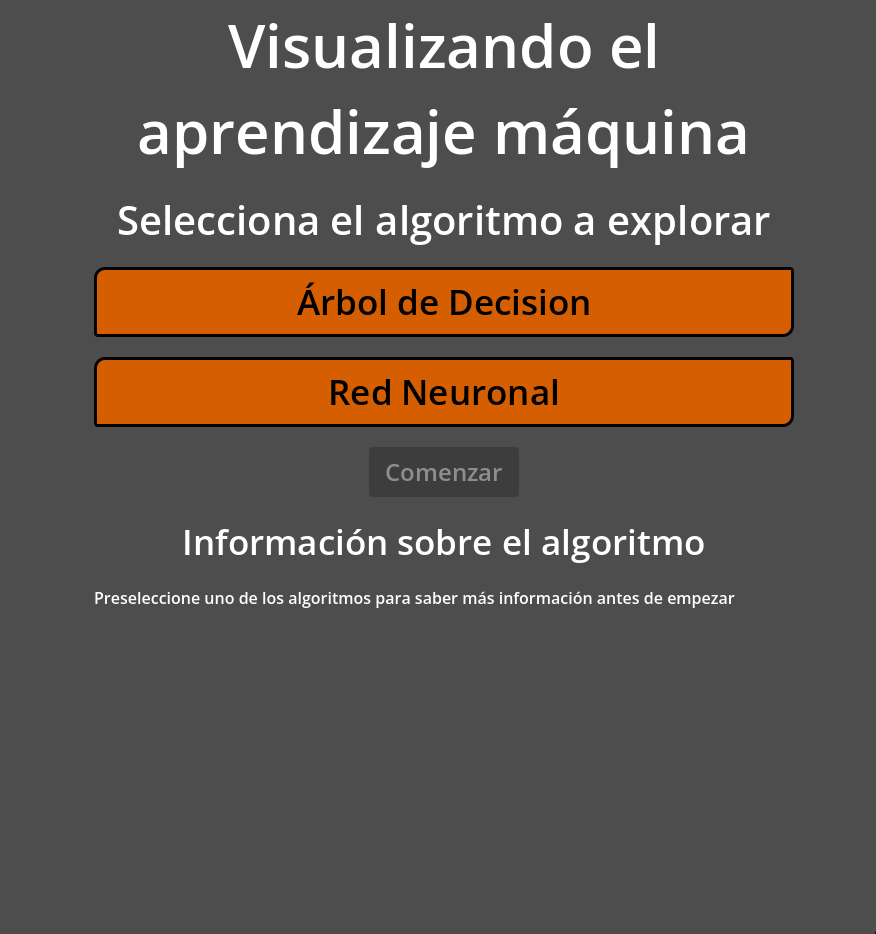
\includegraphics[width=0.7\textwidth]{imaxes/a_mm_2.png}
  \caption{Una de las iteraciones del menú principal.}
  %\label{fig:}
\end{figure}

\begin{figure}[H]
  \centering
  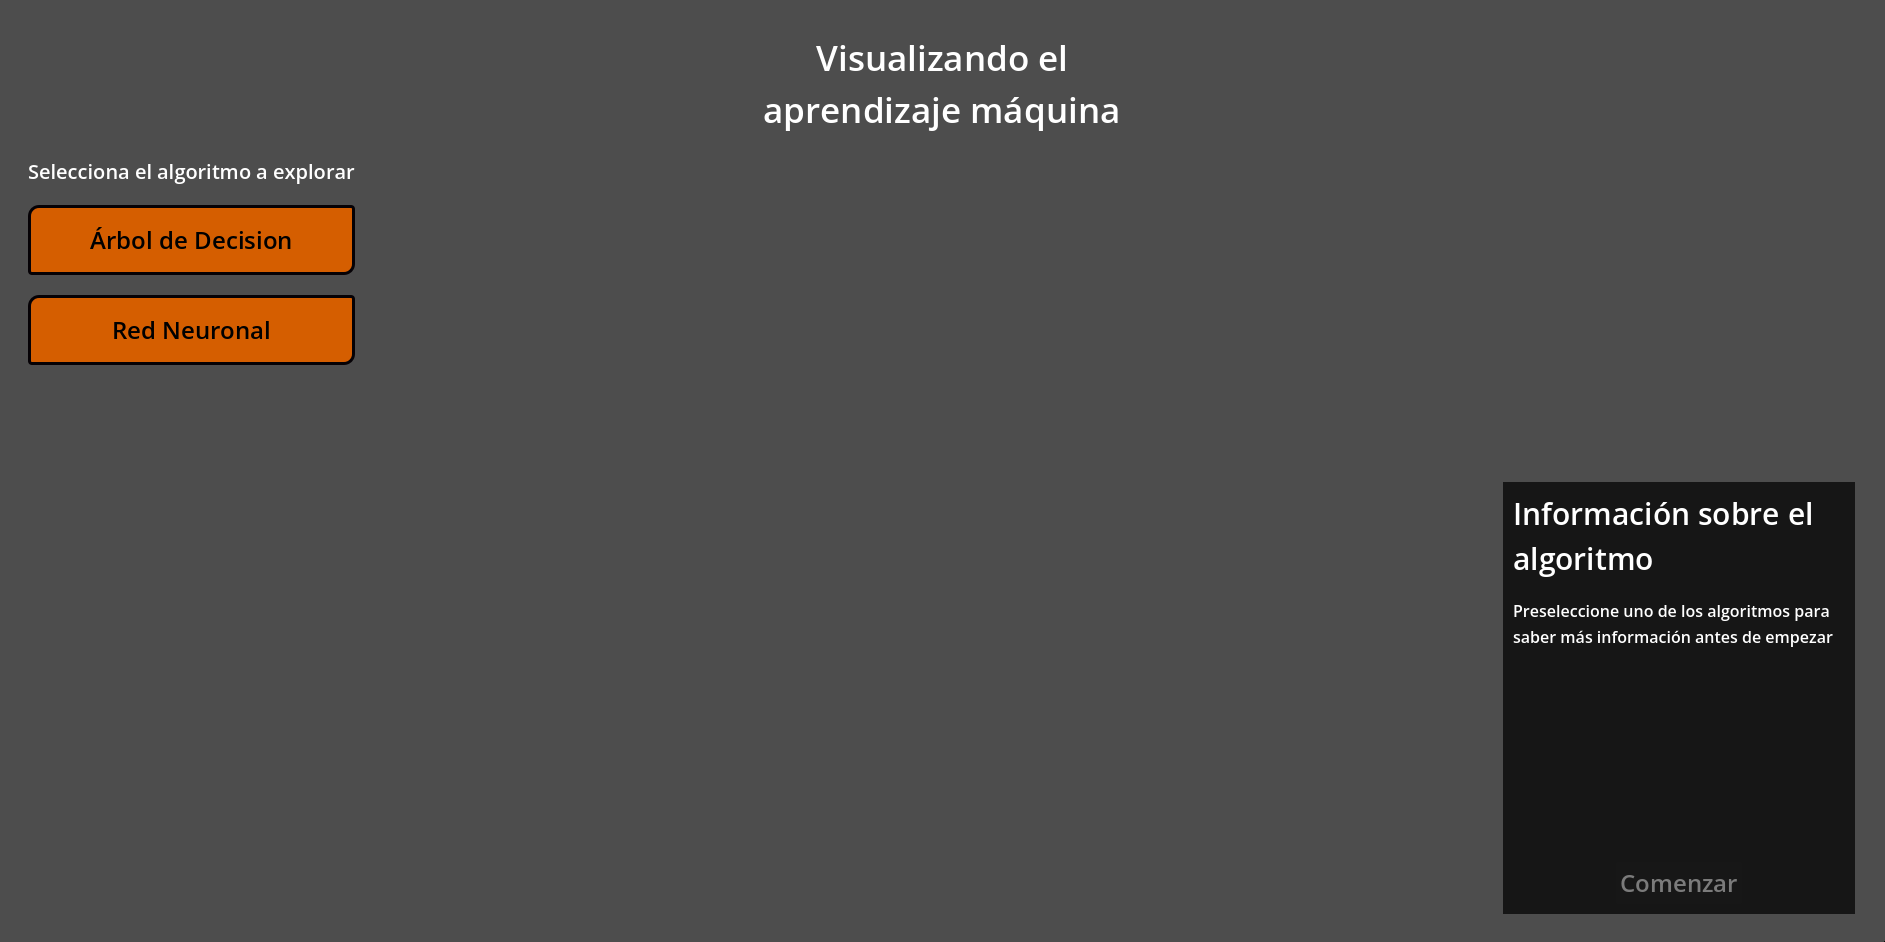
\includegraphics[width=0.7\textwidth]{imaxes/a_mm_1.png}
  \caption{Una de las iteraciones del menú principal.}
  %\label{fig:}
\end{figure}

\begin{figure}[H]
  \centering
  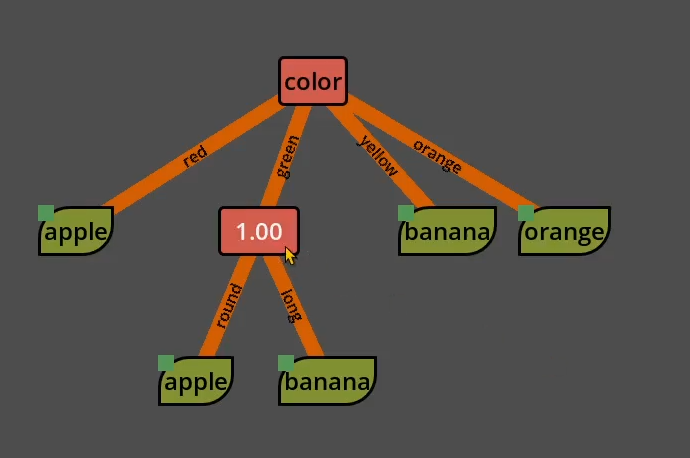
\includegraphics[width=0.7\textwidth]{imaxes/a_numeromal.png}
  \caption{Forma en la que se mostraba la pureza de un nodo en la primera versión.}
  %\label{fig:}
\end{figure}

\begin{figure}[H]
  \centering
  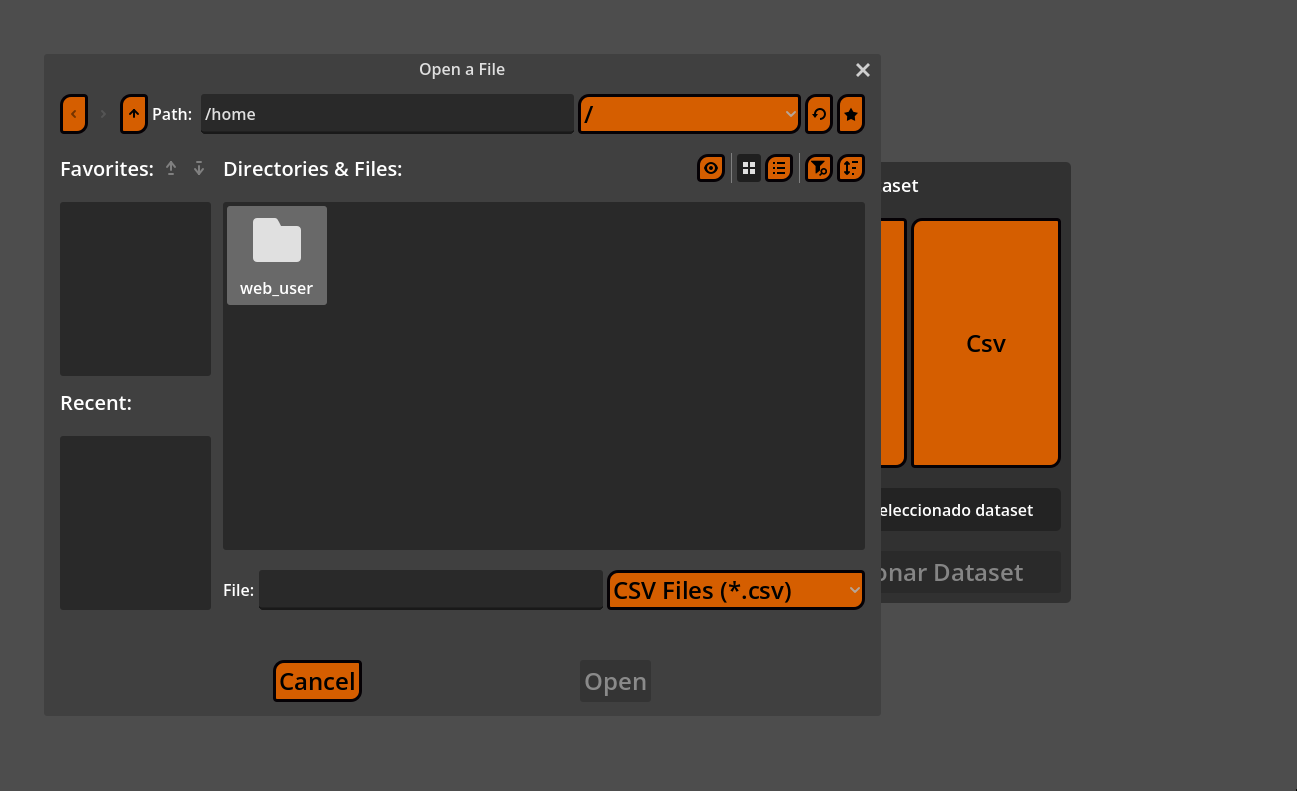
\includegraphics[width=0.7\textwidth]{imaxes/a_menugodot.png}
  \caption{Imagen del menú nativo de Godot que se abría en la versión web antes de crear el puente de JavaScript.}
  %\label{fig:}
\end{figure}
